\section{Notação Visual para WSDL}\label{3-notacao-visual-wsdl}

Uma especificação WSDL pode ser representada graficamente por meio de uma estrutura de grafo. Esta estrutura facilita a compreensão dos diferentes tipos de elementos de uma especificação WSDL, bem como suas relações hierárquicas.

Os tipos de elemento de uma especificação WSDL passíveis de serem representados visualmente em uma estrutura de grafo são: \textit{wsdl:interface}, \textit{wsdl:operation}, \textit{wsdl:input}, \textit{wsdl:output}, \textit{wsdl:infault}, \textit{wsdl:outfault}, \textit{wsdl:fault}, \textit{xs:complexType} e, por fim, \textit{xs:simpleType}. Cada elemento é representado por um nó no grafo. Estes elementos são hierarquicamente dispostos no grafo em um formato de árvore, partindo do elemento mais genérico, \textit{wsdl:interface}, no topo da árvore, até o elemento mais específico, \textit{xs:simpleType}, na base da árvore.

O grafo de uma especificação WSDL é composto por cinco níveis. Os primeiros três níveis do grafo são utilizados para representar a estrutura de interfaces, de operações, de mensagens de entrada, de saída e de falhas de uma especificação WSDL, enquanto que os dois últimos níveis são utilizados para representar os tipos complexos e os tipos simples de dados XSD.

As arestas que ligam elementos (nós) do grafo são representadas por setas. Uma seta origina-se sempre em um elemento mais específico e destina-se a um elemento mais genérico. Tal representação indica a existência de uma relação entre os elementos conectados. Assim, partindo da base da árvore, elementos \textit{xs:simpleType} podem ter arestas destinadas tanto a elementos \textit{xs:complexType} quanto a elementos \textit{wsdl:input}, \textit{wsdl:output} ou \textit{wsdl:fault}. Elementos \textit{xs:complexType} podem ter arestas destinadas tanto a elementos \textit{wsdl:input}, \textit{wsdl:output} e \textit{wsdl:fault} quanto a elementos \textit{xs:complexType} mais genéricos. Elementos \textit{wsdl:fault} podem ter arestas destinadas tanto a elementos \textit{wsdl:infault}, quanto a elementos \textit{wsdl:outfault}. Elementos \textit{wsdl:input}, \textit{wsdl:output}, \textit{wsdl:infault} e \textit{wsdl:outfault} que, por sua vez, podem compôr uma operação, podem ter arestas destinadas, portanto, a elementos \textit{wsdl:operation}. Finalmente, elementos \textit{wsdl:operation} compõem uma interface, resultando em arestas destinadas a \textit{wsdl:interface}, no topo da árvore.

A \figurename~\ref{fig:grafo-wsdl-niveis} ilustra as representações visuais para cada elemento WSDL e XSD, juntamente com os níveis da estrutura hierárquica do formato de árvore. Na lateral esquerda, podemos visualizar as representações visuais dos elementos do grafo juntamente com suas cardinalidades. No centro, podemos visualizar os tipos de elementos WSDL e XSD relacionados às suas representações visuais. Por fim, na lateral direita, podemos visualizar os níveis que definem a estrutura hierárquica do grafo.

\begin{figure}[h]
    %\resizebox{\textwidth}{!}{
    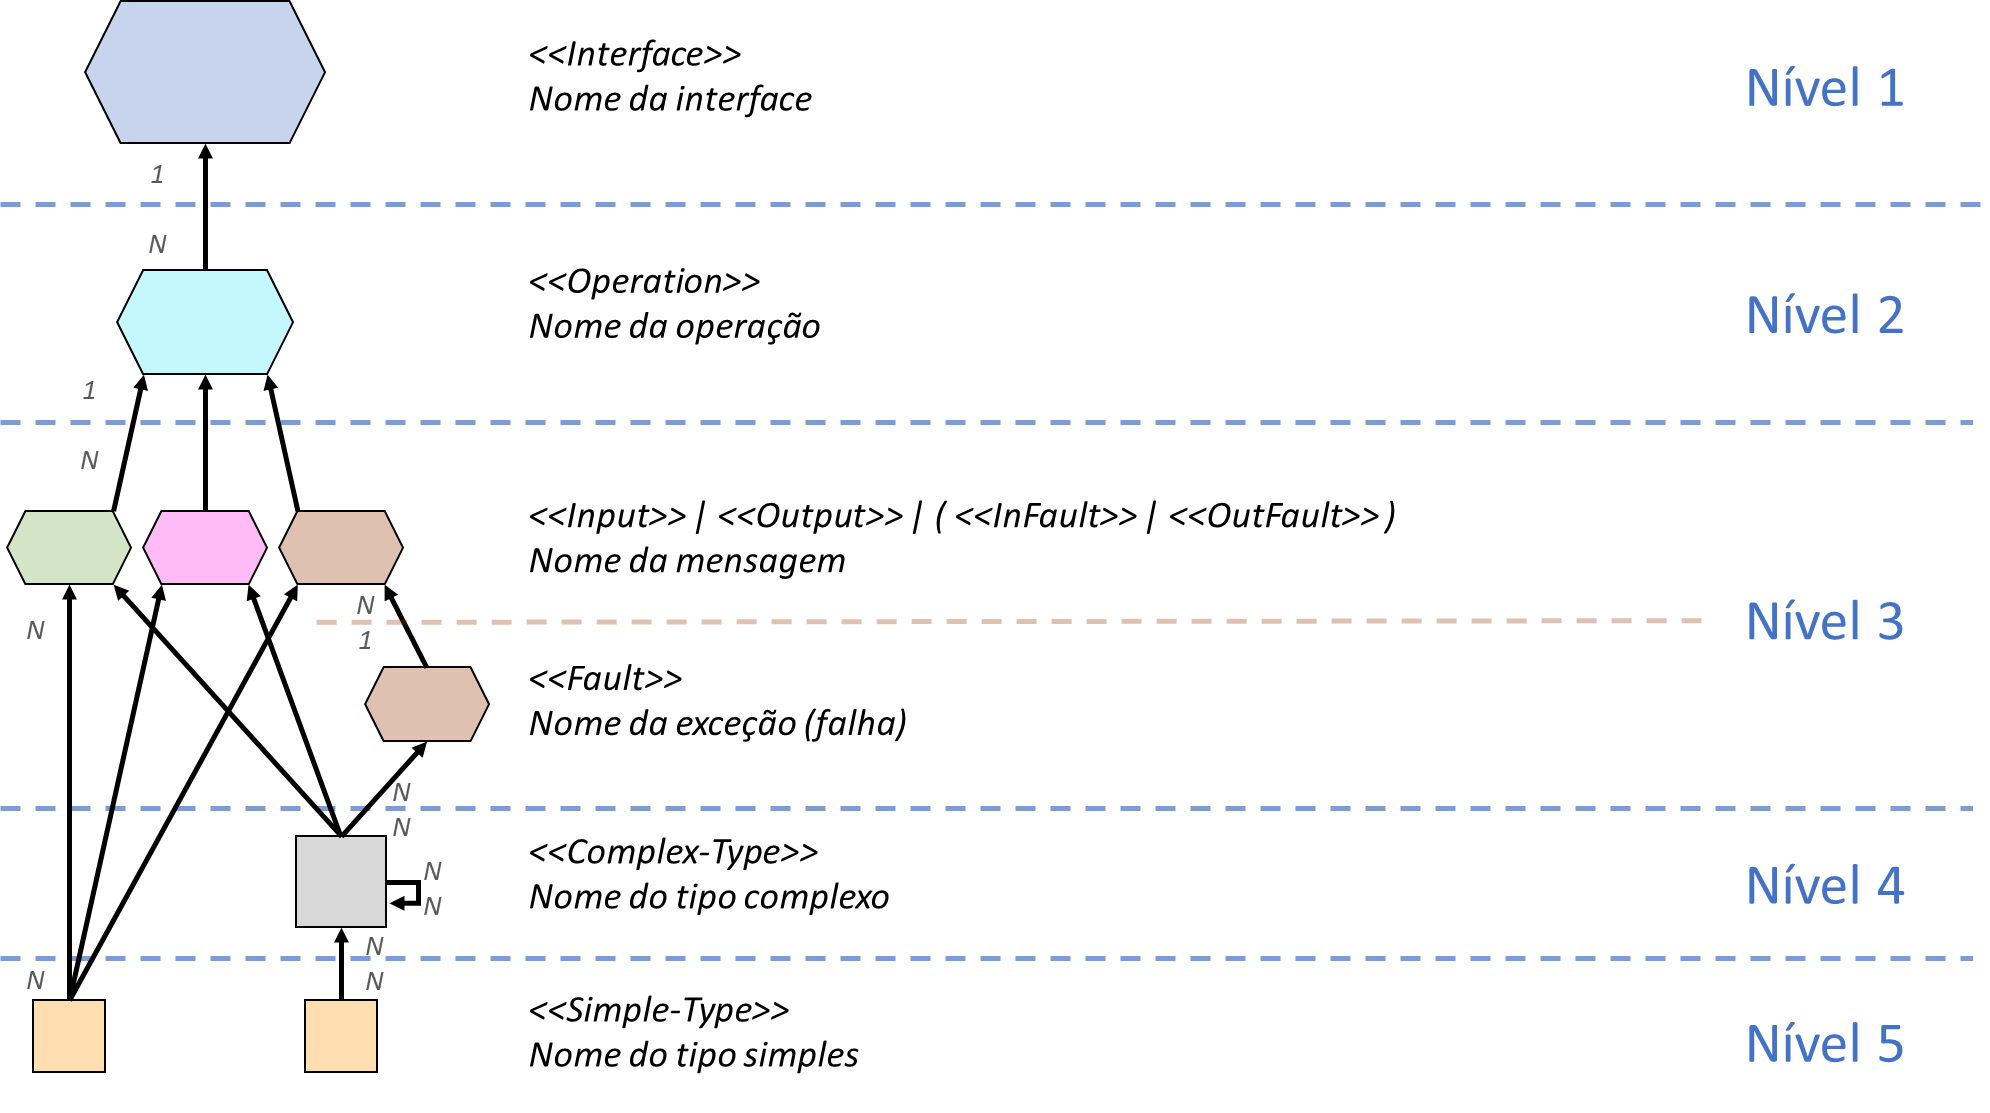
\includegraphics[scale=0.3]{3-notacao-visual-sawsdl/imagens/grafo-wsdl-niveis.PNG}
    %}
    \centering
    \caption[Representações visuais de elementos WSDL]{\textbf{Representações visuais de elementos WSDL.}}
    \label{fig:grafo-wsdl-niveis}
\end{figure}

O quinto nível do grafo (nível 5) consiste da representação visual de elementos XSD do tipo \textit{xs:simpleType}. Estes elementos podem ser utilizados tanto para compor elementos \textit{xs:complexType} quanto para compor elementos \textit{wsdl:input}, \textit{wsdl:output} e/ou \textit{wsdl:fault}. A representação visual de elementos \textit{xs:simpleType} possui o formato geométrico de um quadrado na cor laranja. Dado que estes elementos consistem do último nível do grafo, pode haver arestas partindo destes elementos e destinadas tanto a elementos \textit{xs:complexType} (nível 4) quanto a elementos \textit{wsdl:input}, \textit{wsdl:output} e/ou \textit{wsdl:fault} (nível 3). A cardinalidade dos elementos do quinto nível em relação aos elementos do quarto nível é de N para M (N:M), onde N (nível 5) pode variar entre zero ou várias instâncias (0..*) e M (nível 4) pode variar entre uma ou várias instâncias (1..*). A cardinalidade dos elementos do quinto nível em relação aos elementos do terceiro nível é de N para M (N:M), onde N (nível 5) pode variar entre zero ou várias instâncias (0..*) e M (nível 3) pode variar entre uma ou várias instâncias (1..*). Com isso, pode haver múltiplos elementos no quinto nível relacionados a múltiplos elementos do quarto nível e no terceiro nível. Entretanto, o nível 5 pode ser opcional, pois elementos \textit{xs:complexType} não necessariamente precisam ser estruturados em termos de elementos \textit{xs:simpleType}.

O quarto nível do grafo (nível 4) consiste da representação visual de elementos XSD do tipo \textit{xs:complexType}. Esta representação visual também possui o formato geométrico de um quadrado. Porém, \textit{xs:complexType} possui um tamanho maior em relação aos elementos \textit{xs:simpleType} do nível anterior (nível 5). Adicionalmente, a cor cinza é utilizada para sua representação. Dado que estes elementos consistem do quarto nível do grafo, pode haver arestas partindo destes elementos e destinadas a elementos \textit{wsdl:input}, \textit{wsdl:output} e/ou \textit{wsdl:fault}, no nível 3. Adicionalmente, dado que um elemento \textit{xs:complexType} pode ser composto tanto por outros elementos \textit{xs:complexType} quanto por elementos \textit{xs:simpleType}, podemos ter um número variável de composições, resultando em tantos sub-níveis quantos forem necessários a fim de representar tais composições. Com isso, o nível 4 do grafo poder possuir múltiplos sub-níveis. A cardinalidade dos elementos do quarto nível em relação aos elementos do terceiro nível é de N para M (N:M), onde N (nível 4) pode variar entre uma ou várias instâncias (1..*) e M (nível 3) pode variar entre uma ou várias instâncias (1..*). Assim, pode haver múltiplos elementos no quarto nível relacionados a múltiplos elementos do terceiro nível. Entretando, o nível 4 pode ser opcional desde que o nível 5 esteja presente, pois \textit{wsdl:input}, \textit{wsdl:output} e \textit{wsdl:fault} podem ser exclusivamente compostos por elementos \textit{xs:simpleType}.

O terceiro nível do grafo (nível 3) consiste da representação visual das mensagens de entrada e saída, juntamente com as mensagens de falhas e as definições de exceções tratadas por estas falhas. Com isso, no nível 3, podemos representar os elementos WSDL dos tipos \textit{wsdl:input}, \textit{wsdl:output}, \textit{wsdl:infault}, \textit{wsdl:outfault} e, finalmente, \textit{wsdl:fault}. Estas representações visuais possuem o formato geométrico de um hexágono irregular. Porém, estes elementos se diferem pela cor: a representação de \textit{wsdl:input} possui a cor verde; a representação de \textit{wsdl:output} possui a cor rosa; por fim, a representação dos elementos \textit{wsdl:infault}, \textit{wsdl:outfault} e \textit{wsdl:fault} possui a cor marrom. Os cinco elementos possuem o mesmo tamanho.

Para os elementos \textit{wsdl:input}, \textit{wsdl:output}, \textit{wsdl:infault} e \textit{wsdl:outfault}, há arestas partindo destes elementos e destinadas a elementos \textit{wsdl:operation}, no próximo nível (nível 2). Estas arestas indicam que \textit{wsdl:input}, \textit{wsdl:output}, \textit{wsdl:infault} e \textit{wsdl:outfault} compõem um elemento \textit{wsdl:operation}. Para elementos \textit{wsdl:fault}, pode haver arestas destinadas tanto a elementos \textit{wsdl:infault} quanto a \textit{wsdl:outfault}. Estas arestas indicam que \textit{wsdl:fault} pode compor tanto \textit{wsdl:infault} quanto \textit{wsdl:outfault}. A cardinalidade de elementos \textit{wsdl:input}, \textit{wsdl:output}, \textit{wsdl:infault} e \textit{wsdl:outfault}, do terceiro nível, em relação a elementos \textit{wsdl:operation}, do segundo nível, é de N para 1 (N:1), onde N (nível 3) pode variar entre zero ou várias instâncias (0..*). A cardinalidade de elementos \textit{wsdl:fault} em relação a elementos \textit{wsdl:infault} e \textit{wsdl:outfault}, todos no mesmo nível (nível 3), é de 1 para N (1:N). O nível 3 está sempre presente na estrutura hierárquica de uma especificação WSDL.

O segundo nível do grafo (nível 2) consiste da representação visual de elementos WSDL do tipo \textit{wsdl:operation}. Estas representações visuais também possuem o formato geométrico de um hexágono irregular. Porém, estes elementos são representados na cor ciano e em um tamanho maior em comparação aos elementos do nível anterior (nível 3). Dado que estes elementos consistem do segundo nível do grafo, há arestas originadas nestes elementos e destinadas a um elemento \textit{wsdl:interface}, do próximo nível (nível 1). Estas arestas indicam que elementos \textit{operation} compõem uma \textit{wsdl:interface}. A cardinalidade dos elementos do segundo nível em relação aos elementos do primeiro nível é de N para 1 (N:1), onde N (nível 2) pode variar entre uma ou mais instâncias (1..*). Com isso, pode haver múltiplos elementos no segundo nível, mas eles só podem estar relacionados a um único elemento do primeiro nível. O nível 2 está sempre presente na estrutura hierárquica de uma especificação WSDL.

Por fim, o primeiro nível do grafo (nível 1), topo da árvore, consiste da representação visual de elementos WSDL to tipo \textit{wsdl:interface}. Estas representações visuais possuem o formato geométrico de um hexágono irregular na cor azul. Dado que estes elementos consistem do primeiro nível da árvore, não há arestas originadas deles. O nível 1 também está sempre presente na estrutura hierárquica do grafo WSDL.

Além das diferentes cores, tamanhos e formas, os elementos do grafo são também identificados por textos (estereótipos) posicionados no canto superior esquerdo em relação ao nó do grafo. Para os elementos \textit{wsdl:interface}, o estereótipo \texttt{<<Interface>>} é utilizado. Para os elementos \textit{wsdl:operation}, o estereótipo \texttt{<<Operation>>} é utilizado. Para os elementos \textit{wsdl:input}, o estereótipo \texttt{<<Input>>} é utilizado. Para os elementos \textit{wsdl:output}, o estereótipo \texttt{<<Output>>} é utilizado. Para os elementos \textit{wsdl:infault}, o estereótipo \texttt{<<InFault>>} é utilizado. Para os elementos \textit{wsdl:outfault}, o estereótipo \texttt{<<OutFault>>} é utilizado. Para os elementos \textit{wsdl:fault}, o estereótipo \texttt{<<Fault>>} é utilizado. Para os elementos \textit{xs:complexType}, o estereótipo \texttt{<<Complex-Type>>} é utilizado. Por fim, para os elementos \textit{xs:simpleType}, o estereótipo \texttt{<<Simple-Type>>} é utilizado.

A \figurename~\ref{fig:grafo-wsdl} ilustra o uso da notação proposta para a representação de diferentes elementos da especificação WSDL. Uma inferface \texttt{BookStoreService} é composta pela operação \texttt{GetBook}. Esta operação, por sua vez, é composta pelas mensagens \texttt{GetBookRequest} (entrada), \texttt{GetBookResponse} (saída) e \texttt{BookNotFoundException} (falha de saída). A mensagem de entrada, \texttt{GetBookRequest}, utiliza o tipo de dado complexo \texttt{Book}, que por sua vez é composto pelo tipos simples \texttt{BookName} e \texttt{BookId}. A mensagem de saída, \texttt{GetBookResponse}, utiliza o tipo de dado complexo \texttt{ArrayOfBooks}.  \texttt{ArrayOfBooks} por sua vez utiliza o tipo complexo \texttt{Book}, o qual é composto pelos  tipos simples \texttt{BookName} e \texttt{BookId}. Por fim, a mensagem de falha de saída \texttt{BookNotFoundException} é composta pela falha \texttt{BookNotFoundException}. Esta falha utiliza o tipo complexo \texttt{BookNotFound}, o qual é composto pelo tipo simples \texttt{BookId}.

\begin{figure}[h]
    %\resizebox{\textwidth}{!}{
    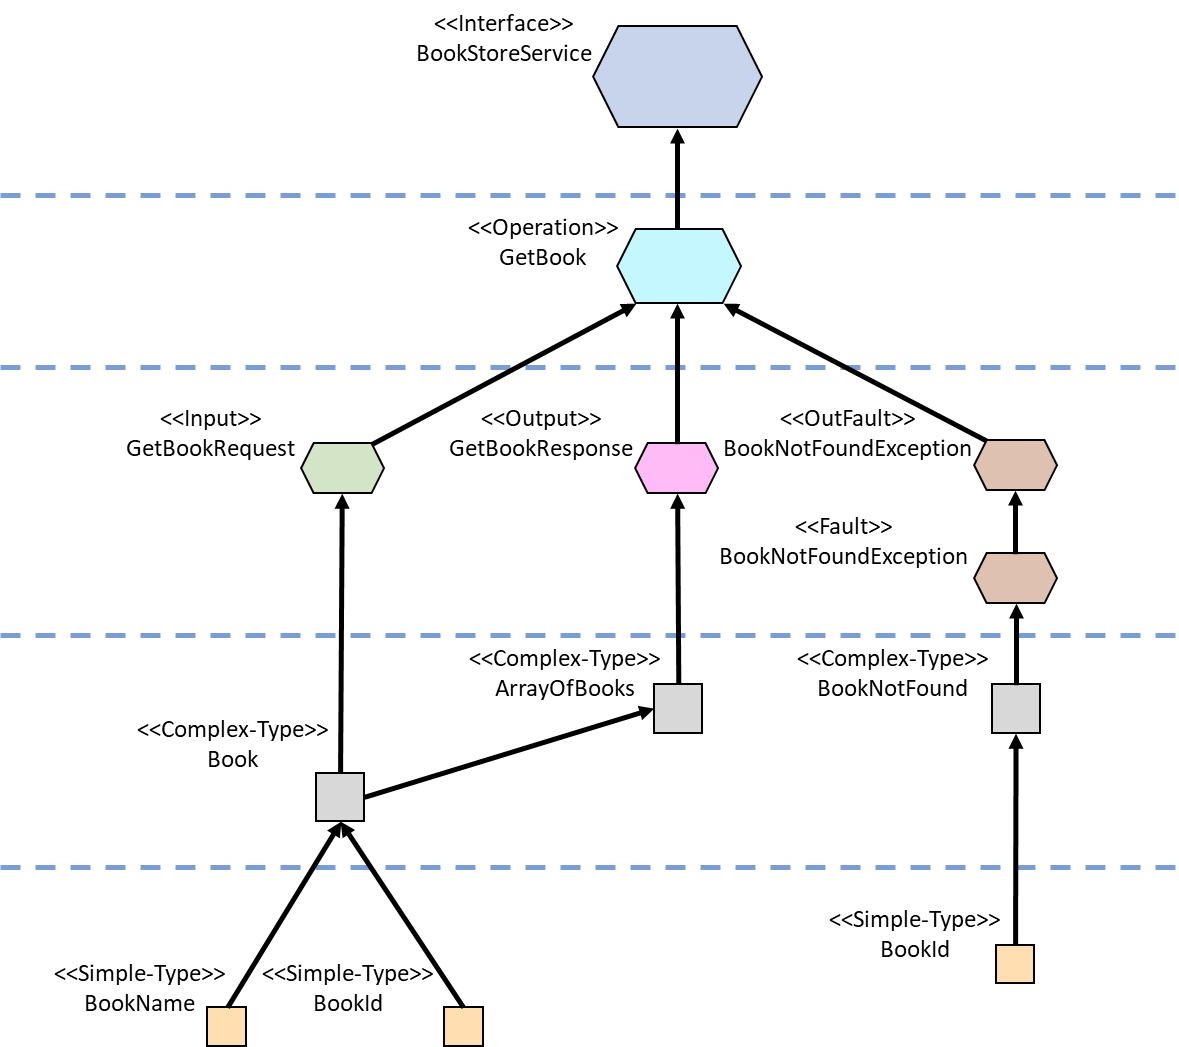
\includegraphics[scale=0.4]{3-notacao-visual-sawsdl/imagens/grafo-wsdl.PNG}
    %}
    \centering
    \caption[Representações visuais de elementos WSDL juntamente com a codificação dupla]{\textbf{Representações visuais de elementos WSDL juntamente com seus estereótipos.}}
    \label{fig:grafo-wsdl}
\end{figure}